% !TEX root = ../../main.tex

\section{Schémas numériques}

\subsection{Méthode de \emph{splitting} haniltonien}
% -------------------------------------------------------------------

Nous utilisons ici une méthode de \emph{splitting} hamiltonien. Pour le modèle $1dz -- 3dv$ celui-ci se décompose en 4 étapes, et il s'écrit sous la forme :
\begin{equation}
  \begin{aligned}
    & \partial_t U = \{ U,\mathcal{H}_{j_c}\} + \{ U,\mathcal{H}_B\} + \{ U,\mathcal{H}_E\} + \{ U,\mathcal{H}_{f_h}\} \\
    & U(t=0) = U_0
  \end{aligned}
  \label{eq:hamsplitting}
\end{equation}

Nous allons nous intéresser au calcul de $\varphi_t^{[j_c]}$, $\varphi_t^{[B]}$, $\varphi_t^{[E]}$ et $\varphi_t^{[f_h]}$ les solutions correspondant à chaque étape de sorte que $\varphi(U_0)$ de~\eqref{eq:hamsplitting} peut être approximé au temps $t$ avec une composition des sous-flux $\varphi_t^{[j_c,B,E,f_h]}$.

\paragraph{Étape $\mathcal{H}_{j_c}$ :\\}
Pour obtenir $\varphi_t^{[j_c]}$, solution du sous-flux $\mathcal{H}_{j_c}$ :
$$
  \begin{cases}
    \partial_t j_{c,\perp} &= -Jj_{c,\perp}B_0 \\
    \partial_t B_\perp     &= 0 \\
    \partial_t E_\perp     &= -j_{c,\perp} \\
    \partial_t f_h         &= 0
  \end{cases}
$$
nous calculons :
$$
  \varphi_t^{[j_c]}(U_0) = \begin{pmatrix}
    e^{-tJ}j_{c,\perp}(0)B_0 \\
    E_\perp(0) - J\left(e^{-tJ}-I\right)j_{c,\perp}(0) \\
    B_\perp(0) \\
    f_h(0)
  \end{pmatrix}
$$
Cela s'obtient car $\int_0^t \exp(-sJ)j_{c,\perp}(0)\,\mathrm{d}s = J\left(\exp(-tJ)-I\right)j_{c,\perp}(0)$.

\paragraph{Étape $\mathcal{H}_B$ :\\}
Nous souhaitons calculer $\varphi_t^{[B]}$, correspondant à la solution du système :
$$
  \begin{cases}
    \partial_t j_{c,\perp} &= 0 \\
    \partial_t B_\perp     &= 0 \\
    \partial_t E_\perp     &= -J\partial_zB_\perp \\
    \partial_t f_h         &= 0
  \end{cases}
$$
qui s'obtient de la manière suivante :
$$
  \varphi_t^{[B]}(U_0) = \begin{pmatrix}
    j_{c,\perp}(0) \\
    E_\perp(0) - tJ\partial_zB_\perp(0) \\
    B_\perp(0) \\
    f_h(0)
  \end{pmatrix}
$$


\paragraph{Étape $\mathcal{H}_E$ :\\}
Pour calculer la solution du sous-flux correspondant à $\mathcal{H}_E$, nous devons résoudre le système suivant :
$$
  \begin{cases}
    \partial_t j_{c,\perp} &= \Omega_{pe}^2E_{perp} \\
    \partial_t B_\perp     &= J\partial_zE_\perp \\
    \partial_t E_\perp     &= (0,0)^\mathsf{T} \\
    \partial_t f_h         &= E_\perp\cdot\nabla_{v_\perp}f_h
  \end{cases}
$$

Avec la conition initiale donnée par $U(t=0)=U_0=(j_{c,\perp},B_\perp,E_\perp,f_h)(t=0)$, la solution au temps $t$ est obtenue par :
$$
  \varphi_t^{[E]}(U_0) = \begin{pmatrix}
    j_{c,\perp} + t\Omega_{pe}^2E_\perp(0)\\
    B_\perp(0)+tJ\partial_zE_\perp(0) \\
    E_\perp(0) \\
    f_h(0,z,v_\perp+tE_\perp(0),v_z)
  \end{pmatrix}
$$
Le calcul de $f_h(0,z,v_\perp+tE_\perp(0),v_z)$ s'effectue en utilisant deux interpolations polynomiale de Lagrange d'ordre 5 à une dimension (une dans la direction $v_x$ et une autre dans la direction $v_y$).

\paragraph{Étape $\mathcal{H}_{f_h}$ :\\}

Pour la dernière étape, nous devons calculer une solution du sous-système :
$$
  \begin{cases}
    \partial_t  j_{c,\perp} &= 0 \\
    \partial_t B_\perp      &= 0 \\
    \partial_t E_\perp      &= \int v_\perp f_h\,\mathrm{d}v\\
    \partial_t f_h          &= -v_z\partial_zf_h + (v_yB_0-v_zB_y)\partial_{v_x}f_h + (-v_xB_0+v_zB_x)\partial_{v_y}f_h + (v_xB_y - v_yB_x)\partial_{v_z}f_h
  \end{cases}
$$
Comme pour la résolution de l'équation de Vlasov-Maxwell (\ref{Li:2019}), ce système ne peut être résolu exactement en temps. Mais en suivant \ref{Li:2019}, nous pouvons subdiviser encore l'hamiltonien $\mathcal{H}_{f_h}$ en $\mathcal{H}_{f_h}=\mathcal{H}_{f_{h,x}}+\mathcal{H}_{f_{h,y}}\mathcal{H}_{f_{h,z}}$, où $\mathcal{H}_{f_{h,\star}}=\frac{1}{2}\int v_{\star}^2 f_h\,\mathrm{d}\textbf{v}$, où $\star=x,y,z$. Cela condtuit à résoudre des sous-système suivant :
\begin{itemize}
  \item $\mathcal{H}_{f_{h,x}}$ :
  \item $\mathcal{H}_{f_{h,y}}$ :
  \item $\mathcal{H}_{f_{h,z}}$ :
\end{itemize}
 

%%%%%%%%%%%%%%%%%%%%%%%%%%%%%%%%%%%%%%%%%%%%%%%%%%%%%%%%%%%%%%%%%%%%%


\subsection{Méthode de Lawson sur le modèle hybride}
% -------------------------------------------------------------------

Dans cette section nous allons présenter la méthode d'intégration exponentielle pour discrétiser le modèle VHL~\eqref{eq:VHM:jx}-\eqref{eq:VHM:fh}. Il est naturel de réécrire ce système, après une transformée de Fourier dans la direction $z$, sous la forme :
$$
  \partial_t U = LU + N(t,U)
$$
où $\kappa=\frac{2j\pi}{N_z}$, $j\in[\![-\frac{N_z}{2},\frac{N_z}{2}]\!]$ représente les modes de Fourier et avec :
\begin{equation}
  L = \begin{pmatrix}
    0   & -B_0 & 0          &  0          &  \Omega_{pe}^2 & 0             & 0 \\
    B_0 &  0   & 0          &  0          &  0             & \Omega_{pe}^2 & 0 \\
    0   &  0   & 0          &  0          &  0             & i\kappa       & 0 \\
    0   &  0   & 0          &  0          & -i\kappa       & 0             & 0 \\
   -1   &  0   & 0          & -i\kappa    &  0             & 0             & 0 \\
    0   & -1   & i\kappa    &  0          &  0             & 0             & 0 \\
    0   &  0   & 0          &  0          &  0             & 0             & -v_z\partial_z \\
  \end{pmatrix},
  \quad
  N:t,U\mapsto \begin{pmatrix}
    0 \\
    0 \\
    0 \\
    0 \\
    \int v_x f \,\mathrm{d}v \\
    \int v_y f \,\mathrm{d}v \\
    E_{\perp}\cdot\nabla_{v_\perp} f - v\times B\nabla_v f
  \end{pmatrix}
  \label{eq:3:LNmaxwell}
\end{equation}
Mais le calcul de la partie linéaire $e^{\tau L}$ nécessaire pour l'écriture du schéma de la méthode LRK n'est pas réalisable avec \sympy{} ou un autre logiciel de calcul formel. Cela vient de l'expression des valeurs propres, dépendant du temps ($\tau$) et de la discrétisation dans l'espace de Fourier des dérivées spatiales ($\kappa\in\left\{\frac{2\pi j}{L},j\in[\![-N_z,N_z]\!]\right\}$). Pour résoudre ce problème, il est décidé dans un premier temps d'intégrer la partie provenant des équations de Maxwell de $L$ dans la partie non-linéaire $N$. Ce qui nous mène à redéfinir $L$ et $N$ comme :
\begin{equation}
  L = \begin{pmatrix}
    0   & -B_0 & 0 &  0 &  \Omega_{pe}^2 & 0             & 0 \\
    B_0 &  0   & 0 &  0 &  0             & \Omega_{pe}^2 & 0 \\
    0   &  0   & 0 &  0 &  0             & 0             & 0 \\
    0   &  0   & 0 &  0 &  0             & 0             & 0 \\
   -1   &  0   & 0 &  0 &  0             & 0             & 0 \\
    0   & -1   & 0 &  0 &  0             & 0             & 0 \\
    0   &  0   & 0 &  0 &  0             & 0             & -v_z\partial_z \\
  \end{pmatrix},
  \ 
  N:t,U\mapsto \begin{pmatrix}
    0 \\
    0 \\
     i\kappa E_y \\
    -i\kappa E_x \\
    -i\kappa B_y + \int v_x f \,\mathrm{d}v \\
     i\kappa B_x + \int v_y f \,\mathrm{d}v \\
    E_{\perp}\cdot\nabla_{v_\perp} f - v\times B\nabla_v f
  \end{pmatrix}
  \label{eq:3:LNsmaxwell}
\end{equation}
Un logiciel de calcul formel, comme \sympy, permet d'obtenir $e^{\tau L}$ pour toute valeur $\tau\in\mathbb{R}$ :
\begin{equation}
\resizebox{.9\hsize}{!}{$
  e^{\tau L} \approx \begin{pmatrix}
  		 \alpha\cos(\theta^-)+\beta\cos(\theta^+) & \alpha\sin(\theta^-)-\beta\sin(\theta^+) & 0 & 0 & \gamma\sin(\theta^-) + \gamma\sin(\theta^+) & -\gamma\cos(\theta^-) + \gamma\cos(\theta^+) & 0 \\
  		-\alpha\sin(\theta^-)+\beta\sin(\theta^+) & \alpha\cos(\theta^-)+\beta\cos(\theta^+) & 0 & 0 & \gamma\cos(\theta^-) - \gamma\cos(\theta^+) &  \gamma\sin(\theta^-) + \gamma\sin(\theta^+) & 0 \\
    0 & 0 & 1 & 0 & 0 & 0 & 0 \\
    0 & 0 & 0 & 1 & 0 & 0 & 0 \\
    -\delta\sin(\theta^-)-\delta\sin(\theta^+) &  \delta\cos(\theta^-)-\delta\cos(\theta^+) & 0 & 0 &  \beta\cos(\theta^-)+\alpha\cos(\theta^+) & \beta\sin(\theta^-)-\alpha\sin(\theta^+) & 0 \\
    -\delta\cos(\theta^-)+\delta\cos(\theta^+) & -\delta\sin(\theta^-)-\delta\sin(\theta^+) & 0 & 0 & -\beta\sin(\theta^-)+\alpha\sin(\theta^+) & \beta\cos(\theta^-)+\alpha\cos(\theta^+) & 0 \\
    0 & 0 & 0 & 0 & 0 & 0 & e^{-ikv_z\tau} \\
    \end{pmatrix}
$}
\end{equation}
avec $\alpha = 0.378732187481834$, $\beta = 0.621267812518167$, $\gamma = 0.970142500145332$, $\delta = 0.242535625036333$, et $\theta^\pm = \frac{\sqrt{2}}{2}\tau\sqrt{9\pm\sqrt{17}}$.

C'est donc à partir de la matrice $L$ sans les termes provenant des équations de Maxwell, et avec le terme non-linéaire $N$, contenant les termes des équations de Maxwell, définis dans~\eqref{eq:3:LNsmaxwell}, que nous allons construire notre premier schéma de Lawson. Il est important d'avoir une formulation explicite de l'exponentielle de la partie linéaire pour construire un schéma en temps efficace. En effet le calcul numérique de l'exponentielle d'une matrice pour une valeur de $\tau$ et de $k$ données est élevé et ne peut être effectuer en amont de la simulation. Le calcul en amont de ces quantités impose une discrétisation en espace donnée, et empêche la mise en place de méthodes à pas de temps adaptatif. Nous verrons par la suite, dans la section~\ref{s3:approx}, une méthode permettant d'intégrer les termes des équations de Maxwell dans la partie linéaire de la méthode de Lawson.

\subsubsection{Filtrage de l'équation de Vlasov}
% ~~~~~~~~~~~~~~~~~~~~~~~~~~~~~~~~~~~~~~~~~~~~~~~~~~~~~~~~~~~~~~~~~~~

L'équation de Vlasov contient le terme $(\vb{v}\times\vb{B}_0)$ qui introduit une condition de CFL restrictive qui peut être outrepassé en utilisant le changement de variable $w=e^{tB_0J}v$, avec $w=(w_x,w_y)^\top$ et $v=(v_x,v_y)^\top$, pour filtrer ce terme en influençant le moins possible le reste du système. Nous introduisons $g(t,z,w,v_z) = f_h(t,z,\exp(-tB_0J)w,v_z)$ avec :
$$
  e^{-tB_0J} = \begin{pmatrix}
    \cos(tB_0) & -\sin(tB_0) \\
    \sin(tB_0) &  \cos(tB_0)
  \end{pmatrix},
  \quad
  J = \begin{pmatrix}
    0  & 1 \\
    -1 & 0
  \end{pmatrix}
$$
alors on a $\exp(-tB_0J)w = \left( \cos(tB_0)w_x - \sin(tB_0)w_y , \sin(tB_0)w_x + \cos(tB_0)w_y \right)^\top$. On peut désormais dériver l'équation sur $g$ :
\begin{equation}
  \partial_t g + v_z\partial_z g - e^{-tB_0J}\vb{E}\cdot\nabla_w g - \mathcal{T}_{\vb{v}}^{[B_0]}g = 0,
\end{equation}
où $\mathcal{T}_{\vb{v}}^{[B_0]}g$ est donné par :
\begin{equation}
  \begin{aligned}
    \mathcal{T}_{\vb{v}}^{[B_0]}g &:= (\vb{v}\times\vb{B})\cdot_{\vb{v}}f_h \\
                                  & = \begin{pmatrix}
                                    \cos(tB_0)w_x - \sin(tB_0)w_y \\
                                    \sin(tB_0)w_x + \cos(tB_0)w_y \\
                                    v_z
                                  \end{pmatrix}
                                  \times
                                  \begin{pmatrix}
                                     B_x \\ B_y \\ 0
                                  \end{pmatrix} 
                                  \cdot
                                  \begin{pmatrix}
                                    e^{-tB_0J}\nabla_w g \\
                                    \partial_{v_z}g
                                  \end{pmatrix} \\
                                  & = \begin{pmatrix}
                                    v_z(-\cos(tB_0)B_y + \sin(tB_0)B_x) \\
                                    v_z(\sin(tB_0)B_y + \cos(tB_0)B_x) \\
                                    (\cos(tB_0)w_x-\sin(tB_0)w_y)B_y - (\sin(tB_0)w_x+\cos(tB_0)w_y)B_x
                                  \end{pmatrix}
                                  \cdot
                                  \begin{pmatrix}
                                    \partial_{w_x}g \\
                                    \partial_{w_y}g \\
                                    \partial_{v_z}g
                                  \end{pmatrix}
  \end{aligned}
\end{equation}
Le changement de variable impacte également l'équation d'Ampère~\eqref{eq:VHM:Ex}-\eqref{eq:VHM:Ey}, l'intégrale du courant des particules chaudes devient :
$$
  \int\vb{v}f\dd{\vb{v}} = \int(e^{-tB_0J}w)g\dd{w}\dd{v_z},
$$
les équations d'Ampère peuvent alors se réécrire comme :
\begin{equation}
  \partial_t E_\perp = -J\partial_z B_\perp - j_{c,\perp} + \int (e^{-tB_0J}w)g\dd{w}\dd{v_z}.
\end{equation}
Les autres équations restent  inchangées.

\subsubsection{Calcul de stabilité avec les équations de Maxwell}
% ~~~~~~~~~~~~~~~~~~~~~~~~~~~~~~~~~~~~~~~~~~~~~~~~~~~~~~~~~~~~~~~~~~~

L'introduction des équations de Maxwell dans la partie non-linéaire de la méthode de Lawson, comme indiquée dans~\eqref{eq:3:LNsmaxwell}, implique une condition de stabilité provenant de ces termes. \Josselin{Il faut dire à un moment que la CFL de Maxwell risque d'être plus restrictive que celle provenant de la partie non-linéaire, car dans $N(U)$ il y a un peu de monde, entre autre on a jamais regardé si une CFL survenait des termes de couplage $\int v_\star f \,\mathrm{d}v$. En même temps le titre de la sous-sous-section parle uniquement de la CFL provenant des équations de Maxwell, la CFL qu'on est obligé de subir car on ne sait pas mettre les équations de Maxwell dans la partie linéaire de Lawson.}

\paragraph{Estimation de la condition de stabilité à partir d'une méthode Runge-Kutta :\\}
Il est possible de faire une première estimation de la condition de stabilité en ne considérant que l'équation :
\begin{equation}\label{eq:3:maxeq}
  \dot{U} = A\cdot U
\end{equation}
avec $U = (B_x,B_y,E_x,E_y)^\top$ le vecteur des seules variables impliquées dans les équations de Maxwell, et $A$ la matrice :
$$
  A = \begin{pmatrix}
    0       &  0       &  0       & i\kappa \\
    0       &  0       & -i\kappa & 0       \\
    0       & -i\kappa &  0       & 0       \\
    i\kappa &  0       &  0       & 0 
  \end{pmatrix}
$$
On souhaite résoudre ce problème avec une méthode de type Runge-Kutta, en effet notre choix de partie linéaire dans la méthode de Lawson pour résoudre le système VMHL nous impose de résoudre les équations de Maxwell via une méthode de type Runge-Kutta. La fonction à intégrer en temps par la méthode Runge-Kutta étant linéaire en $U$, on sait que calculer $U^{n+1}$ par une méthode Runge-Kutta revient à multiplier $U^n$ par la fonction de stabilité de la méthode Runge-Kutta choisie, évaluée en $\Delta tA$. On a donc pour une méthode RK(3,3) :
$$
  U^{n+1} = \left(I + \Delta t A + \frac{\Delta t^2}{2}A^2 + \frac{\Delta t^3}{6}A^3 \right)U^n,
$$
et pour une méthode RK(4,4) :
$$
  U^{n+1} = \left(I + \Delta t A + \frac{\Delta t^2}{2}A^2 + \frac{\Delta t^3}{6}A^3 + \frac{\Delta t^4}{24}A^4 \right)U^n.
$$
On note $p_{(s,n)}$ la fonction de stabilité de la méthode Runge-Kutta à $s$ étages et d'ordre $n$ RK($s$,$n$). On appellera par la suite \emph{matrice d'amplification}, la matrice correspondant à l'évaluation de la fonction de stabilité de la méthode RK($s$,$n$) évaluée en $\Delta t A$. Pour des méthodes de type Runge-Kutta à $s$ étages et d'ordre $n$ explicite on a :
$$
  p_{(s,n)}(\Delta t A) = \sum_{k=0}^n \frac{\Delta t^k}{k!}A^k + \sum_{k=n+1}^s c_k\Delta t^kA^k
$$
Ce qui correspond au développement de l'exponentielle jusqu'à l'ordre $n$, plus des termes supplémentaires si $n\neq s$. Pour estimer la CFL de l'équation~\eqref{eq:3:maxeq}, il faut rechercher les valeurs propres de la matrice d'amplification $p_{(s,n)}(\Delta t A)$ de la méthode choisie. Celles-ci dépendent de $\Delta t$ et de $\kappa$, avec les modes de Fourier $\kappa$ qui dépendent directement de la discrétisation en espace choisie, car $\kappa=\frac{2\pi j}{L}$ avec $j \in[\![-\frac{N_z}{2},\frac{N_z}{2} ]\!]$. Pour trouver la condition de stabilité de cette équation il faut donc trouver le couple $(\Delta t,\kappa)$ permettant de garantir que les valeurs propres de $p_{(s,n)}(\Delta t A)$ soient inférieure à 1.

On rappelle que les valeurs propres de $A$ sont : $i\kappa$ et $-i\kappa$, chacune de multiplicité 2, cela nous permet de déterminer les valeurs propres de $p_{(s,n)}(\Delta t A)$ qui sont :
$$
  \begin{aligned}
    p_{(s,n)}( i\kappa\Delta t) &= \sum_{k=0}^n       i^k\frac{\Delta t^k\kappa^k}{k!} + \sum_{k=n+1}^s       i^kc_k\Delta t^k\kappa^k \\
    p_{(s,n)}(-i\kappa\Delta t) &= \sum_{k=0}^n (-1)^ki^k\frac{\Delta t^k\kappa^k}{k!} + \sum_{k=n+1}^s (-1)^ki^kc_k\Delta t^k\kappa^k
  \end{aligned}
$$
Il s'agit de polynômes en $\Delta t\kappa$ que l'on peut réécrire :
$$
  \begin{aligned}
    p_{(s,n)}( i\kappa\Delta t) &=  \sum_{k=0}^{ \floor{\frac{n}{2}}   }(-1)^k\frac{\Delta t^{2k}\kappa^{2k}}{(2k)!}
                                 + i\sum_{k=0}^{ \floor{\frac{n}{2}}-1 }(-1)^k\frac{\Delta t^{2k+1}\kappa^{2k+1}}{(2k+1)!}\\
                                 &\quad+  \sum_{k=\floor{\frac{n}{2}}+1}^{ \floor{\frac{s}{2}}   } (-1)^k c_{2k}\Delta t^{2k}\kappa^{2k}
                                       + i\sum_{k=\floor{\frac{n}{2}}  }^{ \floor{\frac{s}{2}}-1 } (-1)^k c_{2k+1}\Delta t^{2k+1}\kappa^{2k+1} \\
    p_{(s,n)}(-i\kappa\Delta t) &=  \sum_{k=0}^{ \floor{\frac{n}{2}}   }(-1)^k\frac{\Delta t^{2k}\kappa^{2k}}{(2k)!}
                                 - i\sum_{k=0}^{ \floor{\frac{n}{2}}-1 }(-1)^k\frac{\Delta t^{2k+1}\kappa^{2k+1}}{(2k+1)!}\\
                                 &\quad+  \sum_{k=\floor{\frac{n}{2}}+1}^{ \floor{\frac{s}{2}}   } (-1)^k c_{2k}\Delta t^{2k}\kappa^{2k}
                                       - i\sum_{k=\floor{\frac{n}{2}}  }^{ \floor{\frac{s}{2}}-1 } (-1)^k c_{2k+1}\Delta t^{2k+1}\kappa^{2k+1} \\
  \end{aligned}
$$
où l'on remarque que $p_{(s,n)}(-i\kappa\Delta t) = \widebar{p_{(s,n)}(i\kappa\Delta t)}$, donc $\left|p_{(s,n)}(-i\kappa\Delta t)\right|=\left|p_{(s,n)}(i\kappa\Delta t)\right|$. On peut déterminer la condition de stabilité pourles méthodes RK(3,3) et RK(4,4), c'est-à-dire la valeur de $\Delta t\kappa$ telle que $|p_{(n,n)}(i\kappa\Delta t)|=1$, on obtient ainsi respectivement les valeurs $\frac{\sqrt{3}}{\kappa}$ et $\frac{2\sqrt{2}}{\kappa}$ avec $\kappa = \frac{2j\pi}{L}$, $j\in[\![-\frac{N_z}{2},\frac{N_z}{2}]\!]$.


\paragraph{Estimation de la condition de stabilité à partir d'une méthode de Lawson complète :\\}
Une estimation plus précise de la condition de stabilité dû aux équations de Maxwell peut être calculée en résolvant avec une méthode de Lawson le système :
$$
  \dot{U} = LU + NU
$$
où $U = (j_{c,x},j_{c,y},B_x,B_y,E_x,E_y)^\top$, et $L$ (partie linéaire de la méthode de Lawson) et $N$ (partie considérée comme non-linéaire dans la méthode de Lawson) sont deux matrices données par :
$$  L = \begin{pmatrix}
    0 & -1 & 0 & 0 & 4 & 0 \\
    1 &  0 & 0 & 0 & 0 & 4 \\
    0 &  0 & 0 & 0 & 0 & 0 \\
    0 &  0 & 0 & 0 & 0 & 0 \\
   -1 &  0 & 0 & 0 & 0 & 0 \\
    0 & -1 & 0 & 0 & 0 & 0 \\
  \end{pmatrix},
  \ 
  N = \begin{pmatrix}
    0 & 0 & 0  &  0  &  0  & 0  \\
    0 & 0 & 0  &  0  &  0  & 0  \\
    0 & 0 & 0  &  0  &  0  & ik \\
    0 & 0 & 0  &  0  & -ik & 0  \\
    0 & 0 & 0  & -ik &  0  & 0  \\
    0 & 0 & ik &  0  &  0  & 0  \\
  \end{pmatrix}
$$
Les matrices $L$ et $N$ ne commutent pas, donc la fonction de stabilité de la méthode de Lawson ne peut pas être obtenu comme dans le cas scalaire du chapitre~\ref{chap1}. Il est nécessaire pour chaque méthode de calculer sa fonction de stabilité. Nous n'étudierons ici que les méthodes de Lawson induites par la méthode RK(3,3) de Shu-Osher et celle induite par la méthode RK(4,4) dites classique.

Nous allons commencer l'étude par la méthode RK(3,3) définie par :
$$
  \begin{aligned}
    U^{(1)} &= e^{\Delta tL}U^n + \Delta te^{\Delta tL}NU^n \\
    U^{(2)} &= \frac{3}{4}e^{\frac{\Delta t}{2}L}U^n + \frac{1}{4}e^{-\frac{\Delta t}{2}L}U^{(1)} + \frac{\Delta t}{4}e^{-\frac{\Delta t}{2}L}NU^{(1)} \\
    U^{n+1} &= \frac{1}{3}e^{\Delta tL}U^n + \frac{2}{3}e^{\frac{\Delta t}{2}L}U^{(2)} + \frac{2}{3}\Delta te^{\frac{\Delta t}{2}L}NU^{(2)} \\
  \end{aligned}
$$
On peut calculer la fonction de stabilité de la méthode, on obtient alors :
$$
  \begin{aligned}
    U^{n+1} = \Big[ e^{\Delta tL} &+ \Delta t\left(\frac{2}{3}e^{\frac{\Delta t}{2}L}Ne^{\frac{\Delta t}{2}L}+\frac{1}{6}e^{\Delta tL}N + \frac{1}{6}Ne^{\Delta tL}\right) \\
    & + \frac{\Delta t^2}{2}\left(\frac{1}{3}Ne^{\Delta tL}N + \frac{1}{3}e^{\frac{\Delta t}{2}L}Ne^{\frac{\Delta t}{2}L}N + \frac{1}{3} e^{\frac{\Delta t}{2}L}Ne^{-\frac{\Delta t}{2}L}Ne^{\Delta tL} \right) \\
    & + \frac{\Delta t^3}{6}e^{\frac{\Delta t}{2}L}Ne^{-\frac{\Delta t}{2}L}Ne^{\Delta tL}N \Big]U^n
  \end{aligned}
$$
La matrice d'amplification n'est plus un polynôme, nous nous proposons donc de faire une étude numérique. Pour cela on choisit une discrétisation des modes de Fourier $\kappa\in[\![-27,27]\!]$, et pour les pas de temps $\Delta t\in[0,0.125]$. Pour tout couple de cette discrétisation on calcule numériquement les valeurs propres de la matrice d'amplification, qui sont au nombre de 5, sans compter la multiplicité, que l'on tri par valeur absolue. Cela nous permet de représenter graphiquement, sur la figure~\ref{fig:3:vplrk33}, la plus grande valeur propre en chaque point $(\kappa,\Delta t)$ de la discrétisation. On remarque une symétrie, attendue, entre les modes de Fourier positifs et négatifs, et c'est le mode le plus élevé qui va contraindre le plus notre condition de stabilité entre $\kappa$ et $\Delta t$.
\begin{figure}[h]
  \centering
  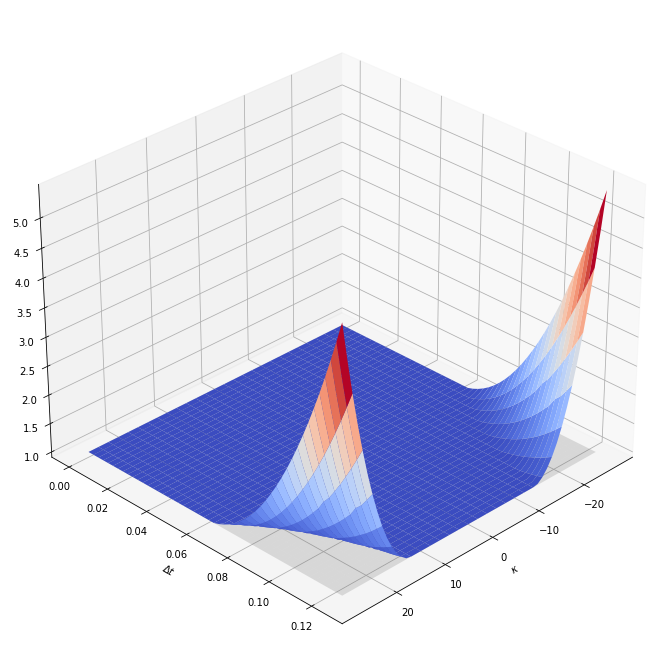
\includegraphics[height=0.49\textheight]{\localPath/figures/vplrk33.png}
  \caption{Plus grande valeur propre en valeur absolue de la matrice d'amplification de la méthode LRK(3,3) sur l'espace discrétisé de $(\kappa,\Delta t)\in[\![-27,27]\!]\times[0,0.125]$}
  \label{fig:3:vplrk33}
\end{figure}
On peut ainsi estimer une condition de stabilité pour $N_z = 15,27$ et on obtient : pour $N_z = 15$, $\Delta t <0.115 \approx \frac{\sqrt{3}}{15}$, et pour $N_z = 27$, $\Delta t <0.066 \approx \frac{\sqrt{3}}{27}$.

On effectue une analyse similaire pour la méthode de Lawson LRK(4,4) suivante :
$$
  \begin{aligned}
    U^{(1)} &= e^{\frac{\Delta t}{2}L}U^n + \frac{\Delta t}{2}e^{\frac{\Delta t}{2}L}NU^n \\
    U^{(2)} &= e^{\frac{\Delta t}{2}L}U^n + \frac{\Delta t}{2}NU^{(1)} \\
    U^{(3)} &= e^{\Delta tL}U^n + \Delta te^{\frac{\Delta t}{2}L}NU^{(2)} \\
    U^{n+1} &= -\frac{1}{3}e^{\Delta tL}U^n + \frac{1}{3}e^{\frac{\Delta t}{2}L}U^{(1)} + \frac{2}{3}e^{\frac{\Delta t}{2}L}U^{(2)} + \frac{1}{3}U^{(3)} \frac{\Delta t}{6}NU^{(3)} \\
  \end{aligned}
$$
Où l'on peut également calculer sa matrice d'amplification :
$$
  \begin{aligned}
    U^{n+1} = \Big[ e^{\Delta t} 
              & + \Delta t\left( \frac{1}{6}e^{\Delta t L}N + \frac{2}{3}e^{\frac{\Delta t}{2}L}Ne^{\frac{\Delta t}{2}L} + \frac{1}{6}Ne^{\Delta t L} \right) \\
              & + \frac{\Delta t^2}{2} \left( \frac{1}{3}e^{\frac{\Delta t}{2}L}Ne^{\frac{\Delta t}{2}L}N + \frac{1}{3}e^{\frac{\Delta t}{2}L}N^2e^{\frac{\Delta t}{2}L} + \frac{1}{3}Ne^{\frac{\Delta t}{2}L}Ne^{\frac{\Delta t}{2}L} \right) \\
              & + \frac{\Delta t^3}{6} \left( \frac{1}{2}e^{\frac{\Delta t}{2}L}N^2e^{\frac{\Delta t}{2}L}N + \frac{1}{2}Ne^{\frac{\Delta t}{2}L}N^2e^{\frac{\Delta t}{2}L} \right) \\
              & + \frac{\Delta t^4}{24}Ne^{\frac{\Delta t}{2}L}N^2e^{\frac{\Delta t}{2}L}N \Big]U^n
  \end{aligned}
$$
Ce qui nous permet, avec la même discrétisation de $\kappa$ et $\Delta t$ de tracer la figure~\ref{fig:3:vplrk44} qui représente la plus grande valeur propre en valeur absolue en chaque point $(\kappa,\Delta t)$ de la discrétisation. Cela nous permet d'obtenir les conditions de stabilité pour différentes discrétisation en espace, et par exemple pour $N_z = 15$ on trouve $\Delta t<0.188 \approx \frac{2\sqrt{2}}{15}$ et pour $N_z = 27$ on trouve $\Delta t < 0.104 \approx \frac{2\sqrt{2}}{27}$.
\begin{figure}[h]
  \centering
  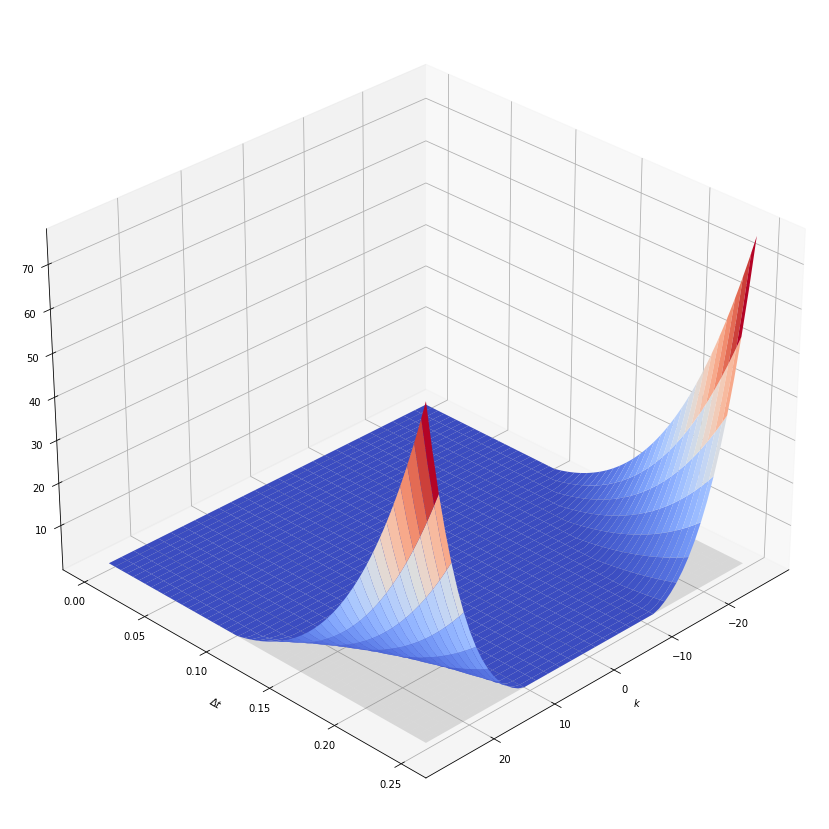
\includegraphics[height=0.49\textheight]{\localPath/figures/vplrk44.png}
  \caption{Plus grande valeur propre en valeur absolue de la matrice d'amplification de la méthode LRK(4,4) sur l'espace discrétisé de $(\kappa,\Delta t)\in[\![-27,27]\!]\times[0,0.125]$}
  \label{fig:3:vplrk44}
\end{figure}
\Josselin{Je ne suis pas nécessairement convaincu par ces 2 figures, qui en plus d'être très similaire visuellement, ne sont pas très lisible. J'ai également tracé la valeur absolue de la plus grande valeur propre en fonction de $\Delta t$ pour différentes valeurs de $\kappa$, j'ai aussi pour un $\kappa$ donné les différentes valeurs propres (et pas que la plus grande). Ce sont des graphiques 2d, sans doute plus lisible, en tout ça ici je trouve ça redondant mais j'attends vos retours pour discuter et savoir ce qui serait mieux}


Cela conclu l'estimation de condition de stabilité en espace. On remarque que l'estimation numérique de la condtion de stabilité de la méthode de Lawson est très proche de la condition de stabilité obtenue à l'aide de la restriction à la résolution de la méthode Runge-Kutta sur $(\vb{B},\vb{E})^\top$.


\subsubsection{Synthèse d'un étage}
% ~~~~~~~~~~~~~~~~~~~~~~~~~~~~~~~~~~~~~~~~~~~~~~~~~~~~~~~~~~~~~~~~~~~

Intéressons nous maintenant à l'implémentation de la méthode de Lawson. Les méthodes de type Runge-Kutta s'écrivent comme une succession d'étage et chaque étage possède des expressions différentes mais une structure similaire. Ces premières sont générées à l'aide d'outils de méta-programmation, présentés dans la sous-section~\ref{ssec:3:codegen}, basés sur la bibliothèque \Python{} de calcul symbolique \sympy{}. Le squelette d'un étage est présent dans l'algorithme~\ref{alg:squeltte}. Celui-ci se comporte en deux grandes sections voir~\ref{alg:l:0} et lignes~\ref{alg:l:15}.

\begin{algorithm}
  \caption{Squelette de l'algorithme d'un étage $s$ d'une méthode LRK}
  \label{alg:squeltte}
  \begin{algorithmic}[1]
    \State{$\triangleright$ Calcul des variables $\hat{j}_{c,x}^{(s)}$, $\hat{j}_{c,y}^{(s)}$, $\hat{B}_{x}^{(s)}$, $\hat{B}_{y}^{(s)}$, $\hat{E}_{x}^{(s)}$ et $\hat{E}_{y}^{(s)}$}\label{alg:l:0}

    \For{$i=0,\dots,N_z$}
      \State $\hat{j}_{h,x,[i]} \gets \sum_{k_x,k_y,k_z} v_{k_x}\,\hat{f}_{h,[i,k_x,k_y,k_z]}^{(s-1)}\,\Delta v$
      \State $\hat{j}_{h,y,[i]} \gets \sum_{k_x,k_y,k_z} v_{k_y}\,\hat{f}_{h,[i,k_x,k_y,k_z]}^{(s-1)}\,\Delta v$
    \EndFor

    \For{$i=0,\dots,N_z$}
      \State $\hat{j}_{c,x,[i]}^{(s)} \gets \dots$ \Comment{les expressions ici sont données par \sympy}
      \State $\hat{j}_{c,y,[i]}^{(s)} \gets \dots$
      \State $\hat{B}_{x,[i]}^{(s)}   \gets \dots$
      \State $\hat{B}_{y,[i]}^{(s)}   \gets \dots$
      \State $\hat{E}_{x,[i]}^{(s)}   \gets \dots$
      \State $\hat{E}_{y,[i]}^{(s)}   \gets \dots$
    \EndFor

    \State
    \State{$\triangleright$ Calcul de la variable $\hat{f}_h^{(s)}$}\label{alg:l:15}

    \State $\left(f\right)_{h,[\cdot,k_x,k_y,k_z]} \gets \textrm{iFFT}_z\left( \hat{f}^{(s-1)}_{h,[\cdot,k_x,k_y,k_z]} \right)$
    \ForAll{ $(k_x,k_y,k_z)\in [\![0,N_x]\!] \times [\![0,N_y]\!] \times [\![0,N_z]\!]$ }
      \For{$i=0,\dots,N_z$}
        \State $a_{v_x} \gets E_{x,[i]} + v_{k_y}B_0 + v_{k_z}B_{y,[i]}$
        \State $a_{v_y} \gets E_{y,[i]} + v_{k_x}B_0 + v_{k_z}B_{x,[i]}$
        \State $a_{v_z} \gets v_{k_x}B_{y,[i]} + v_{k_y}B_{x,[i]}$
        \State $\begin{aligned}\partial_vf_{h,[i,k_x,k_y,k_z]} \gets &\text{WENO}(a_{v_x},f_{h,[i,k_x-3:k_x+3,k_y,k_z]})+\text{WENO}(a_{v_y},f_{h,[i,k_x,k_y-3:k_y+3,k_z]})\\
       &+ \text{WENO}(a_{v_z},f_{h,[i,k_x,k_y,k_z-3:k_z+3]})\end{aligned}$
      \EndFor
    \EndFor

    \ForAll{ $(k_x,k_y,k_z)\in [\![0,N_x]\!] \times [\![0,N_y]\!] \times [\![0,N_z]\!]$ }
      \State $\left(\widehat{\partial_vf}\right)_i \gets \text{FFT}_z(\partial_vf_{\cdot,k_x,k_y,k_z})$
      \For{$i=0,\dots,N_z$}
        \State $\hat{f}_h^{(s)} \gets \dots$ \Comment{l'expression ici est donnée par \sympy}
      \EndFor
    \EndFor
  \end{algorithmic}
\end{algorithm}




